% Uncomment this line for on-screen presentation
\documentclass[xcolor={dvipsnames}]{beamer}\usepackage{etoolbox}\newtoggle{printable}\togglefalse{printable}

% Uncomment this line for printable slides (disable animations and don't waste ink)
%\documentclass[handout, xcolor={dvipsnames}]{beamer}\usepackage{etoolbox}\newtoggle{printable}\toggletrue{printable}

% Adjust these for the path of the theme and its graphics, relative to this file
%\usepackage{beamerthemeFalmouthGamesAcademy}
\usepackage{../../beamerthemeFalmouthGamesAcademy}
\graphicspath{ {../../} }

% Default language for code listings
\lstset{language=C++,
		morekeywords={each,in}
}

\begin{document}
\title{Interface Design \& Evaluation}   
\subtitle{COMP140: Creative Computing Hacking}

\frame{\titlepage} 

\begin{frame}{Lecture Objectives}
	Today's lecture will build upon the practical design of your game controller, focusing on:
	
	\begin{itemize}
		\item Exploring the nature of  input, output, and interaction styles
		\item Examining the role of prototyping in design
		%\item Practical guidelines on one design evaluation technique: heuristic analysis
	\end{itemize}
	
	This will be followed up by a practical in which you will identify heuristics and apply them to a peer's game interface.
\end{frame}

\begin{frame}{Important Notice}
	\begin{columns}[onlytextwidth]
		\begin{column}{0.45\textwidth}
			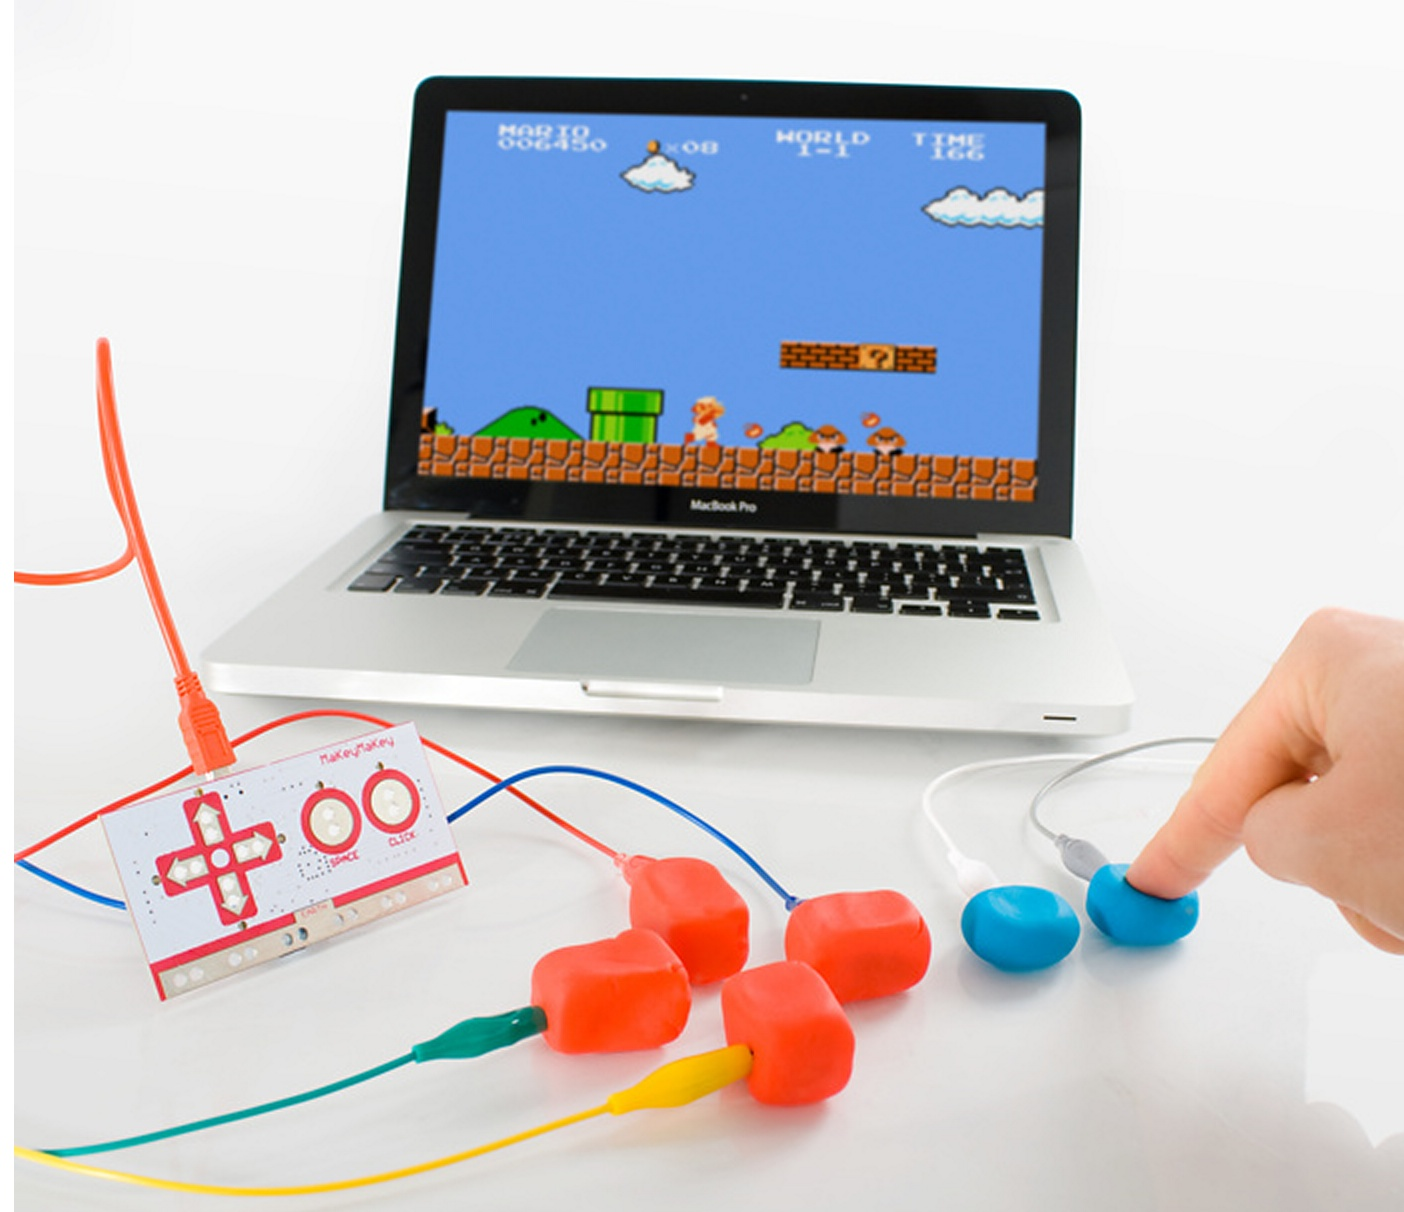
\includegraphics[height=22ex]{MakeyMakey.jpg}
		\end{column}
		\begin{column}{0.45\textwidth}
			Remember to bring your \textit{Makey Makey} kit and associated materials to these lectures for practical 
			support toward the end of each of these sessions.
		\end{column}
	\end{columns}
\end{frame}

\part{Input, Output, and Interaction Styles}
\frame{\partpage}

\begin{frame}{Learning Outcomes}
	In this section you will learn how to...
	
	\begin{itemize}
		\item \textbf{Explain} the role of input and output in systems design
		\item \textbf{List} and \textbf{describe} a variety of input and output devices, giving examples of situations where each may be appropriate
		\item \textbf{Explain} what interaction styles are, while \textbf{critically evaluating} their respective advantages and disadvantages
		\item \textbf{Discuss} the role of direct manipulation in interacting with current computer systems
	\end{itemize}
\end{frame}

\begin{frame}{Further Reading}
	\begin{itemize}
		\item Shneiderman, B. (1998) \textit{Designing the User Interface: Strategies for Effective Human-Computer Interaction}. 3rd Edition. Addison Wesley.
	\end{itemize}
\end{frame}

\begin{frame}{Input and Output Technologies}
	\begin{itemize}
		\item \textbf{input}: the process that occurs as data from the players mind (or from the environment) is transformed into data that computers can use.
		\item \textbf{output}: the process of re-representing computer data into a form the player can perceive, comprehend, and make use of.
	\end{itemize}
\end{frame}

\begin{frame}{Input and Output Technologies}
	When developing and/or selecting an input device for a game, designers are faced with several design trade-offs:
	
	\begin{itemize}
		\item no single optimal device for all tasks 
		\item form of data (e.g. selection verus alphanumeric)
		\item variety of players each with different characteristics
	\end{itemize}
\end{frame}

\begin{frame}{Activity}
	You are making a 2D-platformer for blind players.
	
	\begin{itemize}
		\item Self-organise into pairs.
		\item \textbf{Discuss} the challenges of this scenario on Slack.
		\item \textbf{Research} the characteristics of 2D platformers and blind players, \textbf{posting} your key findings on Slack.
		\item \textbf{Design} and/or \textbf{identify} appropriate an input device to support players' jump accuracy.
	\end{itemize}
	
	\vspace{2ex}
	
	Time: 10-minutes.
\end{frame}

\begin{frame}[fragile]{Socrative \texttt{JBYPC3BBY}}
	\begin{itemize}
		\item \textbf{Summarise} your choice and/or design of input device.
	\end{itemize}
\end{frame}

\begin{frame}{Input and Output Technologies}
	Similar challenges arise when designing and/or selecting output devices for a game:
	
	\begin{itemize}
		\item no single optimal device for all tasks 
		\item form of data (e.g. attention verus conversant)
		\item no single optimal sense to engage
		\item variety of players each with different characteristics
	\end{itemize}
\end{frame}

\begin{frame}{Activity}
	You are making an RTS game for deaf players.
	
	\begin{itemize}
		\item Self-organise into pairs.
		\item \textbf{Discuss} the challenges of this scenario on Slack.
		\item \textbf{Research} the characteristics of RTS games and game players, \textbf{posting} your key findings on Slack.
		\item \textbf{Design} and/or \textbf{identify} appropriate an output device to direct players' attention to units in conflict.
	\end{itemize}
	
	\vspace{2ex}
	
	Time: 10-minutes.
\end{frame}

\begin{frame}[fragile]{Socrative \texttt{JBYPC3BBY}}
	\begin{itemize}
		\item \textbf{Summarise} your choice and/or design of output device.
	\end{itemize}
\end{frame}

\begin{frame}{Interaction Styles}
	\begin{itemize}
		\item \textbf{interaction style}: a term used to describe different approaches to communication between players and computer games.
		\item Includes things such as: 
		\begin{itemize}
			\item command-line entry;
			\item menu;
			\item form-fill;
			\item natural language;
			\item WIMP;
			\item direct manipulation.
		\end{itemize}
	\end{itemize}
\end{frame}

\begin{frame}[fragile]{Socrative \texttt{JBYPC3BBY}}
	\begin{itemize}
		\item In pairs.
		\item Quietly discuss what you think is meant by the acronym `WIMP' for 2-minutes.
		\item \textbf{State} the meaning of WIMP.
	\end{itemize}
\end{frame}

\begin{frame}{Command Line Entry}
	\begin{columns}[onlytextwidth]
		\begin{column}{0.45\textwidth}
			Advantages:
	
			\begin{itemize}
				\item Functionally powerful.
				\item Quick to Use.
			\end{itemize}
		\end{column}
		\begin{column}{0.45\textwidth}
			Disadvantages:
	
			\begin{itemize}
				\item Requires player to remember commands and syntax.
				\item Little feedback, \textit{or} far too verbose.
			\end{itemize}
		\end{column}
	\end{columns}	
\end{frame}

\begin{frame}{Menus}
	\begin{columns}[onlytextwidth]
		\begin{column}{0.45\textwidth}
			Advantages:
	
			\begin{itemize}
				\item Facilittes information navigation.
				\item Restricts potential actions---safe for novices.
				\item Reduces memory load---knowledge in the world.
			\end{itemize}
		\end{column}
		\begin{column}{0.45\textwidth}
			Disadvantages:
	
			\begin{itemize}
				\item Restricts functionality and freedom.
				\item Can be made too complex---difficult to find functions.
			\end{itemize}
		\end{column}
	\end{columns}	
\end{frame}

\begin{frame}{Form Fill-In}
	\begin{columns}[onlytextwidth]
		\begin{column}{0.45\textwidth}
			Advantages:
	
			\begin{itemize}
				\item Paper as a metaphor.
				\item Simple and intuitive.
			\end{itemize}
		\end{column}
		\begin{column}{0.45\textwidth}
			Disadvantages:
	
			\begin{itemize}
				\item Minimally interactive.
				\item Requires an effective supporting layout.
			\end{itemize}
		\end{column}
	\end{columns}	
\end{frame}

\begin{frame}{Natural Language}
	\begin{columns}[onlytextwidth]
		\begin{column}{0.45\textwidth}
			Advantages:
	
			\begin{itemize}
				\item Intuitive and potentially powerful.
				\item Works effectively for simple interactions.
			\end{itemize}
		\end{column}
		\begin{column}{0.45\textwidth}
			Disadvantages:
	
			\begin{itemize}
				\item Technological limitations---accents for example.
				\item Ambiguitiy in language interpretation.
				\item Unsuitable for `twitch' contexts.
			\end{itemize}
		\end{column}
	\end{columns}	
\end{frame}

\begin{frame}[fragile]{Socrative \texttt{JBYPC3BBY}}
	\begin{itemize}
		\item In pairs.
		\item Quietly discuss the advantages of`WIMP' for 2-minutes.
		\item \textbf{State TWO} advantages of WIMP.
	\end{itemize}
\end{frame}

\begin{frame}[fragile]{Socrative \texttt{JBYPC3BBY}}
	\begin{itemize}
		\item In pairs.
		\item Quietly discuss the disadvantages of`WIMP' for 2-minutes.
		\item \textbf{State TWO} disadvantges of WIMP.
	\end{itemize}
\end{frame}

\begin{frame}{Direct Manipulation}
	``The central tenets of direct manipulation are visibility of the objects of interest,
	actions being performed through the rapid, reversible, incremental behaviours and
	actions performed directly on screen objects'' 
	
	\vspace{2ex}
	
	(Perry, 2006, p. 33)
\end{frame}

\begin{frame}{Direct Manipulation}
	Examples:
	
	\begin{itemize}
		\item Interactive Page Animations
		\item Desktop Icons
		\item Scrollbars
	\end{itemize}
\end{frame}

\begin{frame}{Direct Manipulation}
	Direct manipulation aims to address two interface challenges (from Normal and Draper, 1986):
	
	\begin{itemize}
		\item Gulf of Execution
		\item Guld of Evaluation
	\end{itemize}
\end{frame}

\begin{frame}{Gulf of Execution}	
	\begin{itemize}
		\item \textbf{Gulf of execution}: the `distance' between a player's goal and the means of achieving it.
		\item ``One measure of this gulf is how well the system allows the person do the intended actions directly, without extra effort'' (Norman, 1988, p. 51)
	\end{itemize}
\end{frame}

\begin{frame}{Gulf of Evaluation}
	\begin{itemize}
		\item \textbf{Gulf of evaluation}: the `distance' between the state of the game and the player's ability to assess it through perceiving representations.
		\item ``The gulf is small when the system provides information about its state in a form that is easy to get, is easy to interpret, and matches the way the person thinks of the system'' (Norman, 1988, p. 51)
	\end{itemize}
\end{frame}

\begin{frame}{Direct Manipulation}
	Shneiderman (1998) suggests several advantages:
	
	\begin{itemize}
		\item Novices learn functionality quickly  \pause
		\item Experienced users can define new functions and features  \pause
		\item Casual or intermittent users can retain operational concepts  \pause
		\item Built-in constraints mean that all user actions are legal
	\end{itemize}
\end{frame}

\begin{frame}{Direct Manipulation}
	Shneiderman (1998) suggests several advantages:
	
	\begin{itemize}
		\item Change is incremental, with immediate feedback to players \pause
		\item Reduces anxiety because the system is comprehensible and actions reversible \pause
		\item Gain confidence through mimesis and predicting actions
	\end{itemize}
\end{frame}

\begin{frame}[fragile]{Socrative \texttt{JBYPC3BBY}}
	\begin{itemize}
		\item In pairs.
		\item Quietly discuss examples of direct manipulation in games for 2-minutes.
		\item \textbf{State TWO} examples of direct manipulation.
	\end{itemize}
\end{frame}

\part{Prototyping}
\frame{\partpage}

\begin{frame}{Learning Outcomes}
	In this section you will learn how to...
	
	\begin{itemize}
		\item \textbf{Explain} the role of prototyping in game interface design
		\item \textbf{Compare} different approaches to prototyping
		\item \textbf{Select} an appropriate prototyping method for particular usability challenges
	\end{itemize}
\end{frame}

\begin{frame}{Further Reading}
	\begin{itemize}
		\item Jensen, S. (2002) \textit{The Simplicity Shift}. Cambridge University Press.
	\end{itemize}
\end{frame}

\begin{frame}{The Value of Prototyping}
	\begin{itemize}
		\item Jenson (2002) describes the value of prototyping: ``to fail---and fail fast!''
		\item Only by learning from our mistakes can we develop truly usable designs. 
		\item It is very rare, if ever, we get things right the first time and this is especially true of complex systems---such as those in interaction design.
	\end{itemize}
\end{frame}

\begin{frame}[fragile]{Socrative \texttt{JBYPC3BBY}}
	\begin{itemize}
		\item In pairs.
		\item Quietly discuss how prototyping game designs has help you develop those designs, for 2-minutes.
		\item \textbf{Explain} the benefits of prototyping your own words.
	\end{itemize}
\end{frame}

\begin{frame}{Searching the Design Space}
	Design can be conceptualised as serching for an \textit{acceptable} design within an infinite design space. This perspective provokes
	several ideas:

	\begin{itemize}
		\item Designers may not search effectively
		\item Designers may not recognise an \textit{acceptable} design
		\item Designers may converge on a local maxima in the design space: a bad design
	\end{itemize}
\end{frame}

\begin{frame}{Searching the Design Space}
	Prototyping, therefore, becomes:

	\begin{itemize}
		\item An effective search and evaluation method
		\item A means to communicate design information
	\end{itemize}
\end{frame}

\begin{frame}{Searching the Design Space}
	``In practice, prototyping allows designers to \textbf{conceptualise} their products, to better understand the kinds of task that the users do and to
	support them with the appropriate technology''
	
	\vspace{2ex}
	
	(Perry, 2006, p. 50)
\end{frame}

\begin{frame}{Searching the Design Space}
	``Importantly, prototyping forces the [game designers] to visualise all of the steps in [game] software (even beyond the interface), and how well
	the interface will operate in practice.''
	
	\vspace{2ex}
	
	(Perry, 2006, p. 50)
\end{frame}

\begin{frame}[fragile]{Socrative \texttt{JBYPC3BBY}}
	\begin{itemize}
		\item In pairs.
		\item Quietly discuss the consequence of \textbf{not} prototyping and play-testing for 2-minutes.
		\item \textbf{Explain ONE} of these consequences.
	\end{itemize}
\end{frame}

\begin{frame}{Approaches to Prototype Development}
	Prototypes can be used at a number of levels:

	\begin{itemize}
		\item \textbf{Game conceptualisation}: developing the game concept into a game design.
		\item \textbf{Task-level prototyping}: how a particular game mechanic and/or task for the player meshes with player expectation and their attempts to
		fulfill their goals.
		\item \textbf{Menues and HUDs}: the form and placement of data input and output in specific contexts.
	\end{itemize}
\end{frame}

\begin{frame}{Approaches to Prototype Development}
	Different methods facilitate these levels:

	\begin{itemize}
		\item \textbf{Requirements animation}: demonstrating potential functionality and use-cases as animations that can be easily assessed by players. \pause
		\item \textbf{Rapid prototyping}: intensively collecting information on requirements and modelling them as small prototypes that can be easily assessed by players.
	\end{itemize}
\end{frame}

\begin{frame}{Approaches to Prototype Development}
	Different methods facilitate these levels:

	\begin{itemize}
		\item \textbf{Evolutionary prototyping}: developing an initial model that is evaluated and adapted until it `evolves' into an improved end-product.\pause
		\item \textbf{Incremental prototyping}: step-wise development of large prototypes, such as vertical slices, in phases to avoid delays between specification and delivery.
	\end{itemize}
\end{frame}

\begin{frame}{Full Prototype}
	\begin{itemize}
		\item complete version of the intended system
		\item may be a model or a roughly assembled throw-away
	\end{itemize}
\end{frame}

\begin{frame}{Paper Prototype}
	\begin{itemize}
		\item no functionality
		\item used to talk through a design and demonstrate interfaces
	\end{itemize}
\end{frame}

\begin{frame}{Horizontal Prototype}
	\begin{itemize}
		\item complete coverage of the all interface elements
		\item little to no functionality
	\end{itemize}
\end{frame}

\begin{frame}{Vertical Prototype}
	\begin{itemize}
		\item incomplete coverage of the interface elements
		\item high level of functionality in restricted areas
	\end{itemize}
\end{frame}

\begin{frame}{Low Fidelity Prototype}
	\begin{itemize}
		\item little resemblence to the final `look and feel'
		\item cheap and fast to develop
	\end{itemize}
\end{frame}

\begin{frame}{High Fidelity Prototype}
	\begin{itemize}
		\item much resemblence to the final `look and feel' (may even be better i.e., pre-rendered vs real-time in engine)
		\item expensive and time-consuming
	\end{itemize}
\end{frame}

\begin{frame}{`Wizard of Oz' Prototype}
	\begin{itemize}
		\item no functionality at all---simulated through intervention by a hidden person
		\item requires operator to have key knowledge of system states and interactions
	\end{itemize}
\end{frame}

\begin{frame}[fragile]{Socrative \texttt{JBYPC3BBY}}
	\begin{itemize}
		\item In pairs.
		\item Quietly discuss which prototyping appeach is appropriate for early-stage battle interface design for an RPG for 5-minutes.
		\item Prototyping methods are not exclusionary (e.g. could combine high-fidelity with vertical for a pitch).
		\item \textbf{State ONE} prototyping methods \textbf{and justify} your answer.
	\end{itemize}
\end{frame}

\begin{frame}[fragile]{Socrative \texttt{JBYPC3BBY}}
	\begin{itemize}
		\item In pairs.
		\item Quietly discuss which prototyping appeach is appropriate for \textit{late}-stage battle interface design for an RPG for 5-minutes.
		\item Prototyping methods are not exclusionary (e.g. could combine high-fidelity with vertical for a pitch).
		\item \textbf{State ONE} prototyping methods \textbf{and justify} your answer.
	\end{itemize}
\end{frame}

\begin{frame}{Best Practices and Pitfalls}
	Where is prototyping most effective?

	\begin{itemize}
		\item Poorly defined or uncertain requirements
		\item Cost of system rejection is high
		\item High-stakes (think, e.g. nuclear power station)
		\item Assess impact of changes through requirements to implementation (i.e., contract scope)
	\end{itemize}
\end{frame}

\begin{frame}{Best Practices and Pitfalls}
	What are the limitations?

	\begin{itemize}
		\item May introduce uneccessary constraints early in design process
		\item Development has little, if any, direct input by stakeholders (i.e., expert is implementing the prototype)
		\item Consumes time---a trade-off with production schedule
		\item Little data on safety, reliability, response time, and so on---may lead to impractical designs
	\end{itemize}
\end{frame}

\begin{frame}[fragile]{Socrative \texttt{JBYPC3BBY}}
	\begin{itemize}
		\item In pairs.
		\item Quietly discuss which situations are appropriate for prototyping a game component for 2-minutes.
		\item \textbf{Explain ONE} such situation.
	\end{itemize}
\end{frame}

%\part{Usability Evaluation and Heuristic Analysis}
\frame{\partpage}

\begin{frame}{Learning Outcomes}
	In this section you will learn how to...
	
	\begin{itemize}
		\item \textbf{Explain} what heuristic analysis is
		\item \textbf{Recognise} key heuristics for game interfaces
		\item \textbf{Describe} the application of heuristic analysis to game interfaces
	\end{itemize}
\end{frame}

\begin{frame}{Further Reading}
	\begin{itemize}
		\item Nielsen, J. (1993) \textit{Usability Evaluation}. Academic Press.
		\item Pinelle D., Wong N., and Stach, T. (2008) `Heuristic Evaluation for Games: Usability Principles for Video Game Design'. In \textit{Proceedings of the SIGCHI Conference on Human Factors in Computing Systems}. ACM, pp. 1453-1462. 
	\end{itemize}
\end{frame}

\begin{frame}{Usability Evaluation}
	\begin{itemize}
		\item Experts use their knowledge of users and technology to review software usability.
		\item Expert critiques can be formal or informal reports.
		\item Heuristic evaluation is a review guided by a set of heuristics.
		\item A `heuristic' is a mental shortcut that allows people to solve problems and make judgments quickly 
		and efficiently. These rule-of-thumb strategies shorten decision-making time and allow people to function 
		without constantly stopping to think about their next course of action.
	\end{itemize}
\end{frame}

\begin{frame}[fragile]{Socrative \texttt{JBYPC3BBY}}
	\begin{itemize}
		\item In pairs.
		\item Quietly discuss why it is important to `evaluate' a game controller design for 2-minutes.
		\item \textbf{Explain why} evaluation is important in your own words.
	\end{itemize}
\end{frame}


\begin{frame}{Heuristic Analysis}
	\begin{itemize}
		\item Previously, published usability guidelines had hundreds or thousands of rules.
		\item Tended to be inflexible and many rules were context-specific.
		\item HCI scholars desired more fundamental and elegant principles.
	\end{itemize}
\end{frame}

\begin{frame}{Heuristic Analysis}
	\begin{itemize}
		\item In 1990s Jacob Nielsen conducted empirical analyses of key usability challenges.
		\item From this, he and other scholars derived sets of heuristics.
		\item Heuristics tend to be adaptable as technology changes and new evidence is found.
	\end{itemize}
\end{frame}

\begin{frame}{Heuristic Analysis}
Nielsen's (1990) Original Heuristics:

	\begin{columns}[onlytextwidth]
		\begin{column}{0.45\textwidth}
			\begin{itemize}
				\item Simple and Natural Dialogue.
				\item Speak the User's Language.
				\item Minimize memory load.
				\item Consistency.
				\item Feedback.
			\end{itemize}
		\end{column}
		\begin{column}{0.45\textwidth}				
			\begin{itemize}
				\item Clearly Marked Exits.
				\item Shortcuts.
				\item Good Error Messages.
				\item Prevent Errors.
				\item Help and Documentation.
			\end{itemize}
		\end{column}
	\end{columns}
\end{frame}

\begin{frame}{Heuristic Analysis}
Nielsen's (1993) Revised Heuristics:

	\begin{columns}[onlytextwidth]
		\begin{column}{0.45\textwidth}
			\begin{itemize}
				\item Visibility of System Status.
				\item Match Between System and the Real World.
				\item User Control and Freedom.
				\item Consistency.
				\item Error Prevention.
			\end{itemize}
		\end{column}
		\begin{column}{0.45\textwidth}				
			\begin{itemize}
				\item Recognition Over Recall.
				\item Flexibility and Efficiency.
				\item Aesthetic and Minimalist Design.
				\item Help Users Diagnose and Recover from Errors.
				\item Help and Documentation.
			\end{itemize}
		\end{column}
	\end{columns}
\end{frame}

\begin{frame}{Heuristic Analysis}
Shneiderman \textit{et al} (2010) 8 ``Golden'' Rules:

	\begin{columns}[onlytextwidth]
		\begin{column}{0.45\textwidth}
			\begin{itemize}
				\item Strive for Consistency.
				\item Cater to Universal Usability
				\item Offer Informative Feedback.
				\item Design Dialogs to Yield Closure.
			\end{itemize}
		\end{column}
		\begin{column}{0.45\textwidth}				
			\begin{itemize}
				\item Prevent Errors.
				\item Permit Easy Reversal of Actions.
				\item Support Internal Locus of Control.
				\item Reduce Short-Term Memory Load.
			\end{itemize}
		\end{column}
	\end{columns}
\end{frame}

\begin{frame}[fragile]{Socrative \texttt{JBYPC3BBY}}
	\begin{itemize}
		\item In pairs.
		\item Quietly discuss how game controller design for 10-minutes.
		\item \textbf{List ONE} adapted heuristic \textbf{and explain why} it should be included.
	\end{itemize}
\end{frame}

\begin{frame}{Heuristic Analysis}
Pinelle \textit{et al's} (2008) Game Heuristics:

	\begin{columns}[onlytextwidth]
		\begin{column}{0.45\textwidth}
			\begin{itemize}
				\item Consistent Responses to Player's Actions.
				\item Permit Customisation of Game Settings.
				\item Predictable and Reasonable Agent Behaviours.
			\end{itemize}
		\end{column}
		\begin{column}{0.45\textwidth}				
			\begin{itemize}
				\item Provide Manageable Controls with Appropriate Sensitivity and Responsiveness.
				\item Provide Clear Information on Game Status.
				\item Provide Instruction, Training, and Help.
			\end{itemize}
		\end{column}
	\end{columns}
\end{frame}

\begin{frame}{Heuristic Analysis}
Pinelle \textit{et al's} (2008) Game Heuristics:

	\begin{columns}[onlytextwidth]
		\begin{column}{0.45\textwidth}
			\begin{itemize}
				\item Unobstructed Views of Information Needed to Inform Player Actions.
				\item Permit Skipping of Non-Playable Content.
				\item Intuitive and Customizable Input Mappings.
			\end{itemize}
		\end{column}
		\begin{column}{0.45\textwidth}				
			\begin{itemize}
				\item Provide Easily Interpreted Visual Representations
				\item Minimize the Need for Micromanagement.
			\end{itemize}
		\end{column}
	\end{columns}
\end{frame}

\begin{frame}{Heuristic Analysis Method}
	\begin{itemize}
		\item Heuristic evaluation is referred to as `discount' evaluation when 5 evaluators are used
		\item Empirical evidence suggests that on average 5 evaluators identify 75-80\% of usability problems.
	\end{itemize}
\end{frame}



\begin{frame}{Heuristic Analysis Method}
	\begin{itemize}
		\item Select set of heuristics
		\item Brief evaluators
	\end{itemize}
\end{frame}

\begin{frame}{Heuristic Analysis Method}
	\begin{itemize}
		\item Conduct evaluation:
			\begin{itemize}
				\item Each of the 5 evaluators works and takes notes separately.
				\item Each evaluator takes one overall pass of the system to get a feel for it.
				\item Each evaluator takes a second pass to focus on specific features.
				\item If done well, should takes approximately 1-2 hours.
			\end{itemize}
	\end{itemize}
\end{frame}

\begin{frame}{Heuristic Analysis Method}
	\begin{itemize}
		\item Conduct debriefing session:
			\begin{itemize}
				\item The 5 evaluators work together to identify and prioritise problems.
				\item They then report their results collectively to the designer.
				\item If done well, should takes approximately 1 hour.
			\end{itemize}
	\end{itemize}
\end{frame}

\begin{frame}{Heuristic Analysis Method}
Advantages of this approach include (Budd, 2007):

	\begin{itemize}
		\item Few ethical and practical issues as players not involved.
		\item Computing professionals are readily available.
		\item Excellent cost-benefit ratio.
	\end{itemize}
\end{frame}

\begin{frame}{Heuristic Analysis Method}
Disadvantages of this approach include (Budd, 2007):

	\begin{itemize}
		\item Variable quality as best experts require in-depth knowledge of genre and target players.
		\item Important problems are sometimes missed.
		\item Many trivial problems are often identified and over-emphasised.
		\item Experts have biases.
		\item Experts disagree with each other.
	\end{itemize}
\end{frame}

% Move this to next week
%\part{Functions}
\frame{\partpage}

\begin{frame}[fragile]{Function definitions}
    \begin{itemize}
        \item We have already seen an example of a function definition
    \end{itemize}
    \begin{lstlisting}
int main()
{
    std::cout << "Hello, world!" << std::endl;
    return 0;
}
    \end{lstlisting}
    \begin{itemize}
        \item The function \lstinline{main} takes no parameters, and returns a value of type \lstinline{int}
    \end{itemize}
\end{frame}

\begin{frame}[fragile]{Function signatures}
    \begin{itemize}
        \item The \textbf{signature} of a function defines its return type, name, and parameters
    \end{itemize}
    \begin{lstlisting}
double foo(std::string x, int y, bool z)
    \end{lstlisting}
    \pause
    \begin{itemize}
        \item This function takes three parameters: \pause
        \lstinline{x} of type \lstinline{std::string}, \pause
        \lstinline{y} of type \lstinline{int}, \pause
        and \lstinline{z} of type \lstinline{bool} \pause
        \item It returns a value of type \lstinline{double}
    \end{itemize}
\end{frame}

\begin{frame}[fragile]{Functions without return values}
    \begin{itemize}
        \item It is possible to define a function which does not return a value, using the \lstinline{void} keyword
        in place of its return type
    \end{itemize}
    \pause
    \begin{lstlisting}
void printNumber(int n)
{
    std::cout << n << std::endl;
}
    \end{lstlisting}
\end{frame}

\begin{frame}[fragile]{Pass by value}
    \begin{itemize}
        \item Function parameters are passed \textbf{by value}:
        the function receives \textbf{copies} of the original variables
    \end{itemize}
    \pause
    \begin{lstlisting}
void changeName(std::string name)
{
    name = "Ed";
}

int main()
{
    std::string name = "Mike";
    std::cout << name << std::endl; // Mike
    changeName();
    std::cout << name << std::endl; // Mike
}
    \end{lstlisting}
\end{frame}

\begin{frame}[fragile]{Pass by reference}
    \begin{itemize}
        \item Parameters can be passed \textbf{by reference} using \lstinline{&}, allowing the function to modify them
    \end{itemize}
    \pause
    \begin{lstlisting}
void changeName(std::string& name)
{
    name = "Ed";
}

int main()
{
    std::string name = "Mike";
    std::cout << name << std::endl; // Mike
    changeName();
    std::cout << name << std::endl; // Ed
}
    \end{lstlisting}
\end{frame}

\begin{frame}[fragile]{One area where C++ is ``simpler'' than Python!}
    \begin{itemize}
        \item Recall from COMP110 week 6: in Python, basic data types (numbers, booleans, strings etc)
            are passed by value, and object types (lists, dictionaries, class instances) are passed by reference
        \pause
        \item In C++, everything is passed by value unless it is explicitly marked as a reference with \lstinline{&}
    \end{itemize}
\end{frame}

\begin{frame}[fragile]{Constant references}
    \begin{lstlisting}
void greet(std::string name)
{
    std::cout << "Hi " << name << std::endl;
}
    \end{lstlisting}
    \pause
    \begin{itemize}
        \item The string will be copied in order to be passed in \pause
        \item More efficient to pass a reference, and mark it \lstinline{const} to prevent accidental modification
    \end{itemize}
    \begin{lstlisting}
void greet(const std::string& name)
{
    std::cout << "Hi " << name << std::endl;
}
    \end{lstlisting}
    \pause
    \begin{itemize}
        \item (this is only worthwhile for large data structures like strings and vectors, not for basic data types)
    \end{itemize}
\end{frame}



\part{Practical Activity}
\frame{\partpage}

\begin{frame}{Heuristic Analysis Task}
	\begin{itemize}
		\item \textbf{Review} the heuristics at \url{https://www.nngroup.com/articles/ten-usability-heuristics/}.
		\item Self-organise into pairs.
		\item \textbf{Setup} your game and novel game controller.
		\item \textbf{Demonstrate} the prototype to a peer.
		\item \textbf{Conduct} a heurstic analysis of your peer's game interface, following the guidence at:
		\url{https://www.nngroup.com/articles/how-to-conduct-a-heuristic-evaluation/}
	\end{itemize}
\end{frame}

\begin{frame}{Coursework Progress}
	\begin{itemize}
		\item \textbf{Prepare} for the final sprint review to take place next week.
		\item \textbf{Develop} the final draft version of the prototype game controller. 
		\item \textbf{Ensure} that you are ready to conduct heuristic analyses of your peers' work. 
	\end{itemize}
\end{frame}

% -------------------------------------------------------

%\part{The compiler}
%\frame{\partpage}
%
%\begin{frame}
%	\frametitle{The build process}
%	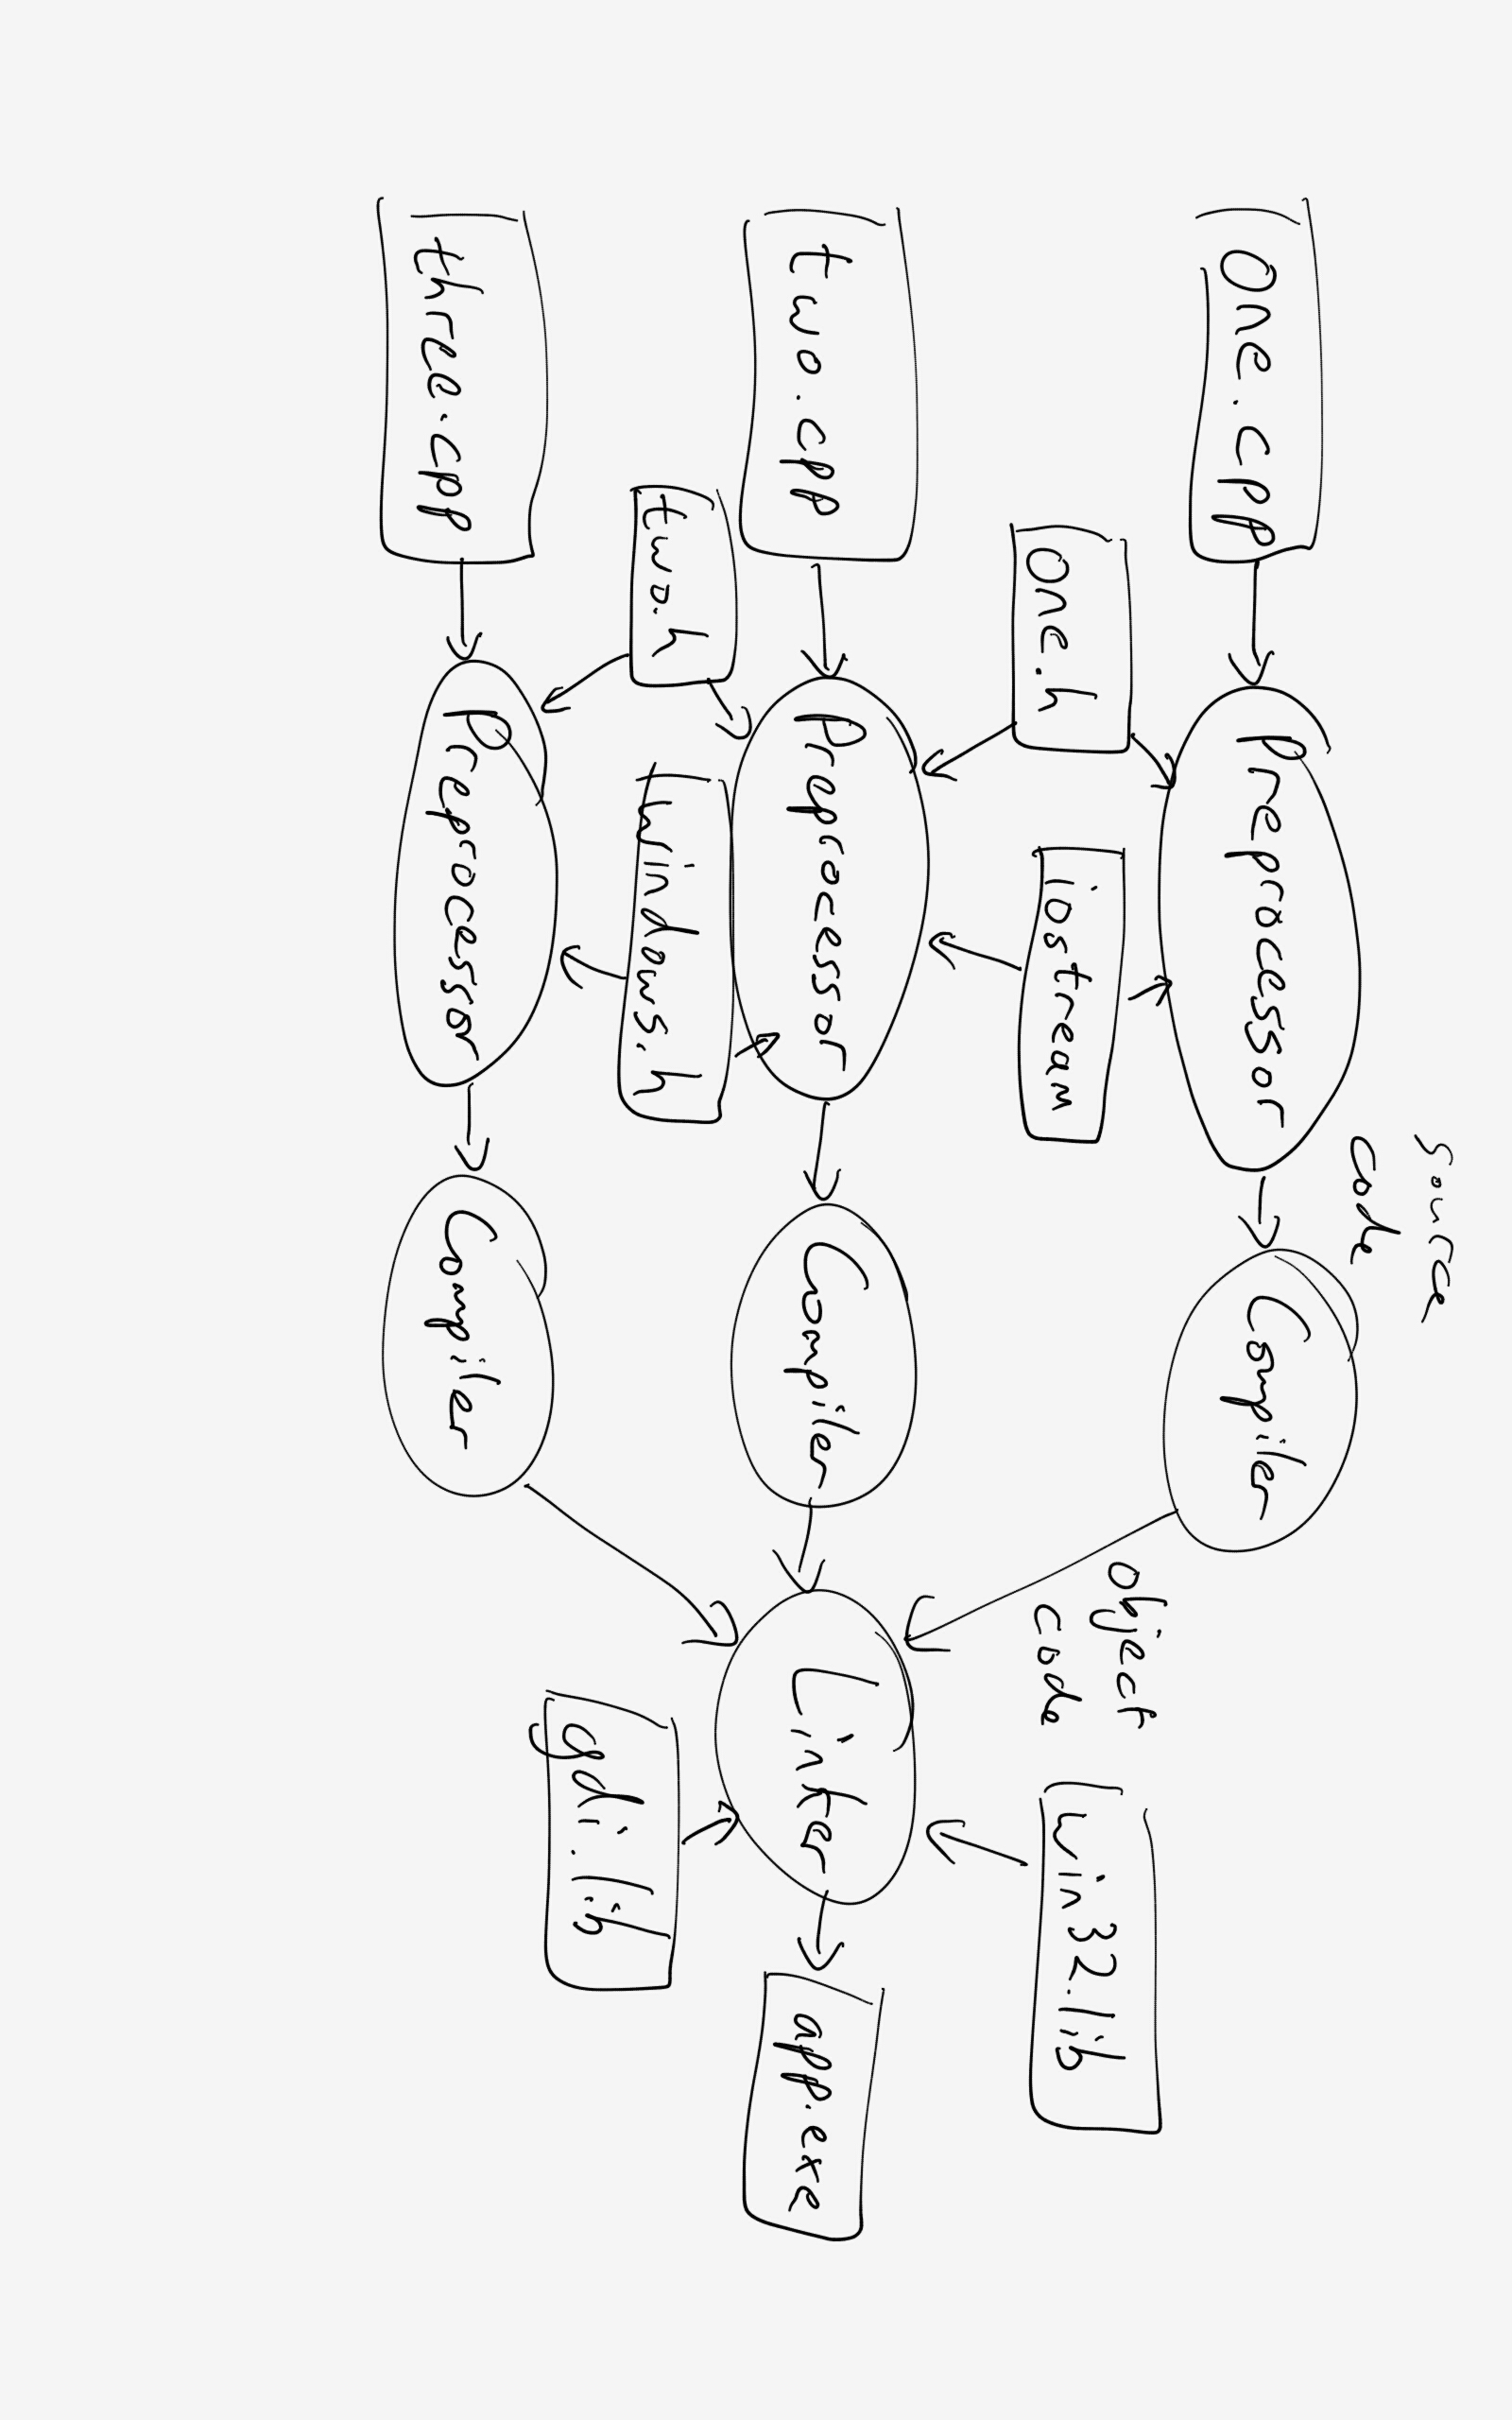
\includegraphics[height=\textwidth,angle=90]{compiler_sketch}
%\end{frame}

\end{document}
